\documentclass{article}
\usepackage[margin=1in]{geometry}
\usepackage{nips13submit_e,times}
\usepackage{hyperref}
\usepackage{url}
\usepackage{graphicx}
\usepackage{amsmath}
\usepackage{color}
\usepackage{listings}

\usepackage{biblatex}
\bibliography{cmput350-paper-bibliography}

\title{CMPUT 350 - TailGate\\
Zerg AI (2013)}

\author{
		Katherine Jasniewski\\
		\texttt{jasiewsk@ualberta.ca} \\
	\AND
		Wyatt Johnson\\
		\texttt{wyatt@ualberta.ca} \\
	\AND
		Thomas Krywitsky\\
		\texttt{krywitsk@ualberta.ca} \\
}

\nipsfinalcopy

\begin{document}

\maketitle

%%%%%%%%%%%%%%%%%%%%%%%%%%%%%%%%%%%%%%%%%%%%%%%%
%%%%%%%% Overview

\section{Project Proposal}

For our original proposal we planned on focusing our efforts on an early game Zergling rush to disrupt the opponent's resource gathering and build order. Mid game we planned on using Hydralisks and Lurkers to attack the opposing team.

Before writing this proposal we had trouble getting the UAlbertaBot running. After getting it running we were able to see how the Zerg AI was implemented. We then thought of a few more things that would more useful to improve upon.

We wanted to make sure hatcheries were being built near our AI’s initial base, instead of the expansion area next to the opponent. We looked through the strategy implemented for the Zerg and realized that the build order was not as well implemented like the Terran and Protoss AI. This became an important improvement we made to our AI.

\section{Prior Experience}

None of our team had experience in AI programming prior to this course. Two team members had played Starcraft 2 but not Starcraft: Brood War. One of our team members was completing a machine learning course at the time of this course, but was unable to implement these features in the final product.

\section{Issues Encountered}

Most of the issues we encountered were related to the lack of support for Zerg within the UAlbertaBot base code. This provided quite a unfair advantage to the other teams as they could simply proceed without worrying about if the units and/or upgrades would work or not.

Our team was unable to get the tournament software working, and thus was only able to produce a small set of statistics rather than what could have been produced.

Another issue we had was our attempts to implement upgrades for our units. We attempted to implement Grooved Spines and Missile Attack upgrades for Hydralisks. Trying to insert these into our code the same way as Terran or Protoss caused our building queue to halt despite there being an abundance of resources and required buildings.

We had trouble getting expansions to build a sufficient amount of drones. During the development of our AI we found that the bot did not handle the amount of drones collecting mineral and gas resources near it expansions. Occasionally one expansion would inherited a drone which collected minerals, though this is too few to make the expansion worth building. As soon as there was an extractor built, there were automatically three drones assigned to collecting gas even in the situations where there was only three drones available, thereby halting mineral collection and effectively losing the game.

Cannot build units while constructing a building. If you choose to construct a building you cannot build units during its construction. This is a problem for rushes because it cripples the bot economy slowing down how fast you can prepare an attack force. This is especially bad for Zerg because we require drones to build buildings and to collect minerals, therefore if we choose to build a building we are short one worker until its completed. This disadvantage leaves Zerg bots with less minerals that Protoss or Terran bots.

\section{Issues Resolved}

\subsection{Build System}
To solve our issue with building support, our team developed a simple searching class/struct that was designed to store dependencies and requirements for the units and upgrades. The biggest issue with this system was the amount factors we had to consider. Reimplementing the base features previously established for the Protoss build order system cause some issues for us in more of a tedious nature rather than complexity.

The build system consisted of three parts, dependencies, and build prerequisites. Some upgrades or units simply require the existence of another (such as the Zergling requiring a Spawning Pool) while others require them as they are consumed (such as a Hatchery needing a drone to use). Implementing this tiered system allowed us to have the flexibility to add in complex goals, and have the build system resolve the dependencies and build prerequisites for us. This not only made it easier for us to write, but gave the AI redundancy if a building or system was destroyed to get it automatically. An example of inserting a Zerg Hydralisk Den is included in \autoref{lst:build_order}.

\begin{lstlisting}[language=c++, frame=single, basicstyle=\footnotesize, caption={Inserting a Build Order}, label=lst:build_order, numbers=left]
static const MetaType map_zerg_spawning_pool(BWAPI::UnitTypes::Zerg_Spawning_Pool);
static const MetaType map_zerg_drone(BWAPI::UnitTypes::Zerg_Drone);
static const MetaType map_zerg_extractor(BWAPI::UnitTypes::Zerg_Extractor);

// Zerg Hydralisk Den
ZergBuildOrder zerg_hydralisk_den(map_zerg_hydralisk_den);

zerg_hydralisk_den.prebuildrequirements.push_back(map_zerg_drone);
zerg_hydralisk_den.dependencies.push_back(map_zerg_spawning_pool);
zerg_hydralisk_den.dependencies.push_back(map_zerg_extractor);

build_order.push_back(zerg_hydralisk_den);
\end{lstlisting}

As seen in \autoref{lst:build_order}, we first create all our ``map'' variables, these map the actual \textit{UnitTypes} to \textit{MetaType}s. We then add the pre-build requirements and the dependencies. These are added as c++ vectors for ease of access. It should now be clear that adding any additional units will require some work to evaluate their needs before we can simply add them to the queue whilst the built in search is not working for Zerg.

\subsection{Drone Production}
We resolved the issue of not being able to implement upgrades by placing more emphasis on dependency resolution for the queue. Checks were inserted to verify that if a upgrade item was added, to verify that it was not already building, or was already built before proceeding to add it to the queue.

The problem with building a sufficient amount of drones was resolved by implementing a smart rebuild option for the drones into the strategy manager. Each call to the \textit{getZergBuildOrderGoal} performs the following check:

\begin{align}
    D_B = \frac{D_H H - D}{4} + 1
\end{align}

Where $D_B$ is the number of drones to build, $H$ is the number of currently built hatcheries, $D_H$ is the number of drones per hatchery wanted (i.e. $8$), $D$ is the number of drones (built/building). This staggers the insertion of drones to prevent over saturating the build queue. While taking some time to rebuild, this static placement seemed to ensure that even if drones were consumed for building, that they would be replaced on the next build queue.

\subsection{Tournament Software}

We were able to get the tournament software working, with some advice from teachers assistants, after our presentation. It still had problems and crashed but we think that the results from it are decently representative of what our bot is capable of.

\section{Statistical Analysis}

We performed our tournament running 10 matches round robin to determine the best overall winner.

\begin{figure}[h]
	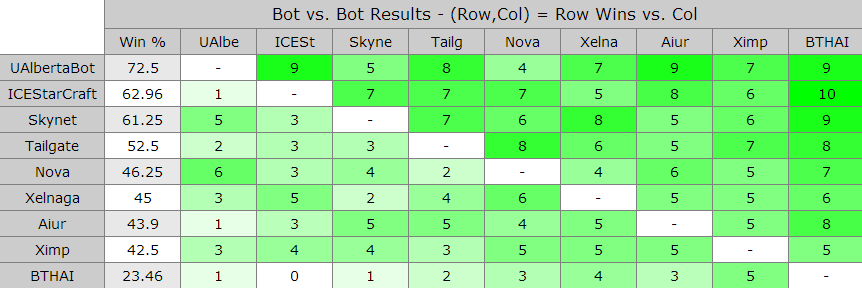
\includegraphics[width=\textwidth]{images/results-by-bot.png}
	\caption{Results By Bot Vs. TailGate}
    \label{fig:results_by_bot}
\end{figure}

Based on the results obtained from testing yielded the results as seen in \autoref{fig:results_by_bot}. Our AI came out $4^{\text{th}}$ overall. What we would have hoped for is to beat the UAlbertaBot (Playing as Protoss), but unfortunately, we were unable to modify our strategy to match the early game defenses that UAlbertaBot put up.

% TODO: INSERT STAT ANA

\begin{figure}[h]
	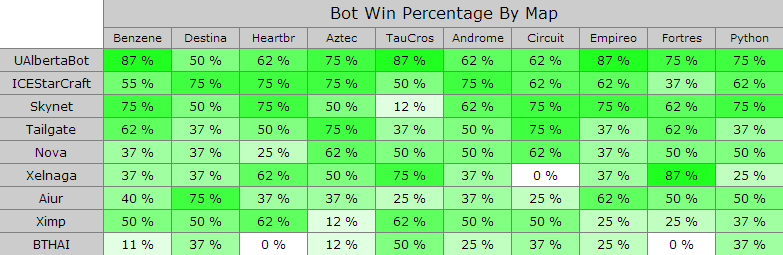
\includegraphics[width=\textwidth]{images/results-by-map.png}
	\caption{Results By Map Vs. TailGate}
    \label{fig:results_by_map}
\end{figure}

The statistics generated using the tournament software \cite{tournament_software} (as seen in \autoref{fig:results_by_bot} and \autoref{fig:results_by_map}) were ran on an earlier revision of the code base, but shared enough of the base characteristics to still be relevant to the current revision. Most of the games won through the tournament software were done as an early game rush. Specifically, the 4 Pool rush still seems to surprise most of the enemy AI's in these tests we ran. After the tournament software was run, we did develop some more solid late game code, but as most matches were very short with ours anyways, we feel that it shouldn't sway results too much.
\section{Motivations for Our Work}

We saw that the initial AI had trouble expanding and gaining control over the map. When the original bot attempted to expand it would build its expansion next to the opponent's base, thereby allowing the opponent to destroy it early on in the game. We thought that expanding properly would allow us to better the AI significantly.

The strategy implemented by the original AI was purely to spawn an initial amount of Zerglings to rush the opponent and stop production entirely. Seeing this we thought that we could make the AI more successful by controlling when it should be spawning Zerglings and other units. 

Our goal was to eliminate the problems Zerg had in its original implementation, and introduce a basic strategy.  

\section{Strategies Implemented}

Our team ended up tinkering with the initial opening book for Zerg to implement common early game tactics. These tactics were selected based on the research we conducted. Maps size, and the race of the opposing team where large factors to determine which strategy we should use.

Specifically, the opening books included use of a 4 Pool Zergling Rush, 5 Pool Zergling Rush, and a 9 Pool Zergling Rush (See \autoref{fig:9poolrush} for an example). The ``X-Pool'' Zergling Rush relates to the number of the drones that turn into the Spawning Pool. The Spawning Pool allows Zerg larvae to transform into Zerglings. As clearly seen in the picture however, the resources are quite stressed, only having $34$ minerals and no gas. This is a typical for a early rushing Zerg player, but it makes it much more difficult to recuperate if the initial rush fails.

\begin{figure}[!ht]
    \centering
	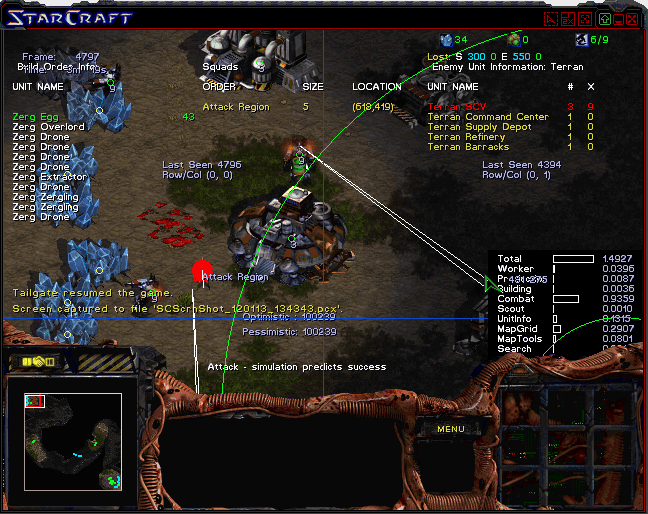
\includegraphics[width=\textwidth]{images/tailgate_ai.png}
	\caption{TailGate AI Finishing a 9 Pool Rush \cite{9poolvprotoss}}
	\label{fig:9poolrush}
\end{figure}

In Starcraft Brood War, there one possible strategy is a 4 Pool Zergling Rush which is the most aggressive of the ``all in'' strategies implemented \cite{4poolrush}. This strategy holds no guarantees of late game progression, but if implemented swiftly, can result in winning on smaller maps within 56 seconds \cite{9poolvprotoss}.

For larger maps, and for Protoss players (Who tend to go for a 2 Gateway rush vs Zerg), we opted to select the 9 Pool Zergling Rush. This provides a stronger force against the opponent earlier on in the game.

\section{Advantages and Disadvantages of our Strategy}

\subsection{Advantages}
An advantage of our strategy is that can be executed quickly. Being able to execute quickly allows us to cripple the opponent earlier on in the game delaying them from achieving their strategy.

Our AI can adjusts itself based on the initial conditions of the map size and the race of the opponent. By making these adjustments we are able to choose the ideal strategy.

We were able to develop a strategy that works fairly well mid-game. By building units with a diverse range of attack types we were able balance them to better counteract the opponents units. With our AI developing and adaptation against the units the opponent is building we gain an advantage.

\subsection{Disadvantages}
Our AI still relies on building placement that was integrated in the original bot code.This is not suitable for Zerg because we can only build on creep. Therefore building placement is scattered rather than controlled to optimize defenses and movement speed.

The ability for our bot to recover and survive into mid-game depends heavily on the strategies our AI chooses to make and the beginning. Rushes take a lot of resources that are critical for mid-game success.

No game to game learning is implemented for our bot. If other bots we face have learning implemented we are at a disadvantage because they will be able to adjust to our strategies.

\section{Future Improvements}

In the future we hope to develop our AI bot to have a working late game strategy, allowing it to stand up against human players as well as bots. Due to the rushing style of our tactics we do not currently take any steps toward a late game push therefore leaving our AI vulnerable. 

We would also like to implement a micromanaging system for our units in particular Zerglings and Mutalisk. We hope that improving the micromanaging of these units in the future will allow us to avoid attacks and splash damage. Micromanaging would also help us control when we want our units to use abilities. Adding focus on units such as Mutalisks allows them to target individual units without getting stuck on bunkers or other fortified structures/units which can easily take them out.

Need to work on controlling where buildings are placed within the base to optimize defences. Rather than randomly building defensive building in our base we hope to make the AI building them near the front of the base to better defend it. To do this successfully we need to overcome the disadvantage that Zerg can only build buildings on creep. Creep being the organic matter which covers the maps terrain and is emitted from certain Zerg buildings.

An original plan our team had was to take advantage of the Burrow ability that some Zerg units were able to obtain through upgrades. We want to use burrow on the opponents base to remain hidden and ambush their units. We thought this might be a good way to disrupt the opponent's economy further by burrowing Lurkers near their workers, since Lurkers are able to attack while burrowed.

We were also hoping to take advantage of lurkers burrowing abilities and sunken colony’s by placing them in choke points by our base. Units planning to attack our base will be quickly confronted by our ranged defenses.

In the future we hope for our AI to take advantage of our extractor building occupying the enemies gas. Using a drone we would occupy the enemys extractor early game so that they would not be able to harvest any gas. We hope to do this by almost building the extractor and then cancelling the build process and then building it again. If the building is being attacked during it’s construction process we can stop construction. The drone will re appear at full health and then we could start construction again. This strategy would require us to reserve enough minerals to continuously build the extractor and will only work early game to slow the enemies gas collection. 

We also hope to implement an extractor trick to overcome population limits. If our population is full early game we can use a drone to build an extractor at our base and queue up and extra Zergling (which produces two Zerglings). As soon as the Zerglings are done building we can stop extractor construction, which gives back our drone, allowing us to get into an overpopulated state. This can be advantageous early game when we plan to rush the enemy.

In the future we would like to customize kiting movement for ranged units. Ranged units can take advantage of kiting other units because they can pause to shoot and continue to run away. This improvement would allow such units as Hydralisks and Mutalisks to avoid getting hit while doing damage to the opponents units. 

\section{Conclusion}

Our team was able to fulfill most of the goals we have proposed in our project proposal. We managed to develop a bot that can run a variety of strategies against the opponent based the maps size, and versing race. We experienced many problems due to the lack of Zerg implementation in the original bot but overcame most of them. We were able to fix a build order system that allows us to make a balanced rush attack and still build mid game units to fortify our base and diversify our army. Running our AI against previously use tournament AI we were able to achieve surprising results that revealed advantages and disadvantages of our strategy. There are still many improvements we would like to make to our bot, that allow us to implement micromanaging tactics, utilizing abilities, place building more effectively and learning which strategies are most effective from previous matches. 

%%%%%%%%%%%%%%%%%%%%%%%%%%%%%%%%%%%%%%%%%%%%%%%%
%%%%%%%% References

\printbibliography

\end{document}
